\chapter{Grundlagen und Verwandte Arbeiten}

Dieses Kapitel beschreibt verwandte Arbeiten und die Grundlagen von Erklärbarkeit sowie dessen Zusammenwirkung mit zusammenhängenden NFRs.

\section{Erklärungen in erklärbaren Systemen}
\label{02_basics:explainable_system}

Erklärbarkeit als Qualitätsaspekt behandelt das Integrieren von Erklärungen in erklärbare Systeme und die damit verbundenen Auswirkungen auf die Softwarequalität. Der Aspekt wird von unterschiedlichen Autoren durch verschiedene Synonyme beschrieben. \citeauthor{brennen_what_2020} hat einen Katalog zusammengestellt, welcher einige Synonyme zusammenfasst \cite{brennen_what_2020}. Dieser enthält unter anderem die Begriffe
% \textit{Accountability}, \textit{Trust}, 
\textit{Transparency}, \textit{Understandability} und \textit{Interpretability}. In der jüngeren Vergangenheit haben verschiedene Autoren diese Begriffe mit differenzierten Bedeutungen in einen Zusammenhang mit \textit{Explainability} gestellt \cite{chazette_end-users_nodate,chazette_knowledge_nodate,kohl_explainability_2019,wang_integration_2020}.

\textit{Transparency} wird als der Grad, zu dem ein System Einblick in dessen Funktionsweise gewährt, beschrieben \cite{chazette_end-users_nodate}. Diese Offenlegung kann dabei verschiedene Aspekte von Systemen wie zugrundeliegende Algorithmen z.~B. in Empfehlungssystemen \cite{balog_measuring_2020} oder trainierte Modelle des Maschinellen Lernens \cite{sovrano_modelling_2020} betreffen.

Das Verstehen von Erklärungen wird unter \textit{Understandability} zusammengefasst \cite{do2010software}. Das so erlangte Verständnis von Systemnutzern ist folglich als subjektiver Einflussfaktor für Erklärungen zu werten \cite{chazette_end-users_nodate}. Für diesen subjektiven Faktor nutzen \citeauthor{wang_integration_2020} sowie \citeauthor{balog_measuring_2020} den Begriff \textit{Perceived Transparency} als Synonym, um die subjektive Aufnahme von \textit{Transparency} bei verschiedenem Verständnis durch Nutzer zu verdeutlichen \cite{wang_integration_2020, balog_measuring_2020}.

Während \textit{Interpretability} zum Teil mit \textit{Understandability} gleichgesetzt wird \cite{chazette_end-users_nodate}, nimmt die Verwendung des Begriffs für den Grad der möglichen Interpretation der Ausgaben von ML-Algorithmen zu \cite{doshi2017towards}.

Da der Fokus dieser Arbeit auf externen Qualitätsaspekten liegt, ist die \textit{Interpretability} von ML-Algorithmen kein Bestandteil dieser Arbeit. Um trotz dessen einer Irritation durch doppelt belegte Begriffe vorzubeugen, wird für den subjektiven Faktor des Verständnisses von Softwaresystem \textit{Perceived Transparency} verwendet.

\bigskip

Welche Rolle spielen nun Erklärungen beim Verstehen von Systemen? Diese Frage 

mental model: \cite{chi_three_nodate}

We consider an explanatory narrative as a sequence of information (explanans) to increase understanding over explainable data and processes (explanandum), for the satisfaction of a specified explainee that interacts with the explanandum having specified goals in a specified context of use. \cite{sovrano_modelling_2020}

Informationen geben \cite{wang_integration_2020}

Specifically, an explanation of a plan in this framework satisfies conditions (1) and (2) below: 1. An explanation is an update to the human mental model 2. such that there is no better plan in the updated mental model than the given plan. Clearly, from the perspective of the model of a planning problem, (1) can be in terms of one or more of • beliefs of the agent about the current state (as opposed to what the human may be aware of); • their actual desires or goals (as opposed to that ascribed to it by the human); • preconditions and effects of actions (as opposed to its capabilities known to the human). 3. Minimally Complete Explanation (MCE) is the shortest model explanation that satisfies (1) and (2). \cite{zahedi_towards_2019}

\textit{Perceived Transparency} \cite{wang_is_2018,balog_measuring_2020}

\glqq Through clear definitions and motivation, the contribution of the evaluation becomes more apparent. \grqq{} \cite{waa_evaluating_2021} \cite{chazette_knowledge_nodate} geben die. erster Ansatz von \cite{kohl_explainability_2019}

Definition 3 (Explainability Requirement): A system S must be explainable for target group G in context C with respect to aspect Y of explanandum X. \cite{kohl_explainability_2019}

\subsection{Erklärbarkeit als Nicht-Funktionale Anforderung}
\label{02_basics:explainability}

\smallskip

\noindent\fbox{
    \parbox{0.964\textwidth}{
        \smallskip
        A system \textbf{S} is explainable with respect to an aspect \textbf{X} of \textbf{S} relative to an addressee \textbf{A} in context \textbf{C} if and only if there is an entity \textbf{E} (the explainer) who, by giving a corpus of information \textbf{I} (the explanation of \textbf{X}), enables \textbf{A} to understand \textbf{X} of \textbf{S} in \textbf{C}.
        \smallskip
    }
}

\smallskip

Abgrenzung: Explainability: Top-Down, Interpretability: Bottom-up understanding \cite{thomson_knowledge--information_2020}. Auch understandability hier abgrenzen

Woraus Erklärungen bestehen können können wird in dieser Arbeit u.~a. beschrieben

NFRs sind ... \cite{chung2009non, schneider2012abenteuer}

\citeauthor{kohl_explainability_2019} hat ...

\citeauthor{chazette2020explainability} challenges

\citeauthor{chazette_end-users_nodate} $\rightarrow$ zweischneidiges schwert

\subsection{Externe Qualitätsziele für Erklärbarkeit}
\label{02_basics:quality_quaracteristic}

Verschiedene SIGs z.B. \cite{do2010software}

\citeauthor{chazette_knowledge_nodate} $\rightarrow$ Auswirkungen auf Qualitätsaspekte

“Evaluating the quality of explanations is traditionally difficult due to their inherent subjectivity. The needs of different user groups can be very different, which is reflected in their expectations of what an explanation should offer.” \cite{martin_developing_2019, martin_evaluating_2021}

\section{Qualitätsmodelle}
\label{sec:basics_quality_models}

Diese Arbeit entwickelt zwar kein Qualitätsmodell für Erklärungen, gibt allerdings Basis für einige Aspekte und benutzt es später auch.

\begin{figure}[htb!]
    \centering
    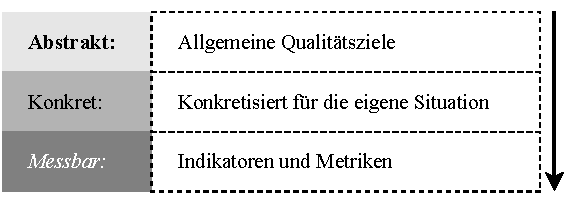
\includegraphics{contents/02_basics/res/quality_models.pdf}
    \caption{Aufbau eines Qualitätsmodells in drei Ebenen \cite[S. 34, ][]{schneider2012abenteuer}}
    \label{fig:basics_quality_models}
\end{figure}

\cite{schneider2012abenteuer}